\begin{chapter}{Background \label{Ch:background}}
This thesis aims to develop tools to aid computationally expensive analyses that a subjective Bayesian may perform. These computationally expensive tasks usually amount to computing $Y = f(\bX)$ where $f(\cdot)$ is an expensive to evaluate function, which is thought to be highly non-linear, $\bX$ is an uncertain vector of inputs to $f(\cdot)$ and $Y$ is the (uncertain) quantity of interest. We consider two concrete instances of such a problem.

The first problem we consider is a sensitivity analysis to aid the elicitation of $\bX$. The sensitivity analysis relies on calculating the intractable integrals $\E_X\{f(\bX)\}$, $\var_X \{f(\bX)\}$, as well as conditional expectations and variances, such as $\E_{X_i} \{  \var_{\bX_{-i}}(f(X) \mid X_i) \}$, where $\bX_{-i}$ denotes all elements of $\bX$ apart from the $i$th element. This in turn relies on evaluation of $f(\bx)$ for many values of $\bx$. The word `many' is somewhat vague, but we would expect that evaluating $f(\cdot)$ at somewhere in the region of $10^4$ -- $10^6$ unique input configurations to be necessary to obtain accurate estimates of the required expectations and variances.

The second problem we consider is decision analysis, in which we elicit a function of the form $U(\bx) = \E_{\btheta} \{ u(\bx, \btheta) \}$ where $\btheta$ is a collection of unknown quantities, $\bx$ is the vector representing the decision to be made, and $u$ is a function which itself depends on $f(\bx)$. This problem is computationally intractable; evaluation of $U(\bx)$ is typically only achievable via Monte Carlo methods. This makes maximising $U(\bx)$ difficult because $U(\bx)$ itself cannot be computed exactly. The difficulty of an intractable decision analysis is increased when $U(\bx)$ is expensive to compute, which is a problem we have.

We will perform analyses on the computationally expensive Athena simulator, which is a stochastic model of an offshore wind farm \citep{Zit13, Zit16, Zit2021}. This chapter will consist of primers on the Athena simulator (\cref{sec:athena}), probability elicitation (\cref{sec:prob}), and  Bayesian decision analysis, including the elicitation of utility functions.

\section{The Athena simulator: a stochastic model of an offshore wind farm\label{sec:athena}}
% some information about the athena simulator
The Athena simulator \citep{Zit13, Zit16, Zit2021} is a point process model of a large offshore wind farm. The intended purpose of Athena is to aid decision making under uncertainty, as such, Athena does not model raw power output or take into account precise details of the wind, but aims to model the reliability of a wind farm using techniques from reliability analysis. The reason for not modelling raw output or including synthetic weather data is that they are highly uncontrollable and very uncertain, although their aggregate effects can be characterised much more precisely. We can however, make plausible predictions about the \textit{reliability} of the wind farm.

The Athena simulator generates predictions by simulating events within an offshore wind farm over a pre-specified time period $[0, T_{max}]$ years. There are many types of event that may happen within an offshore wind farm. Typical events include components breaking, components being repaired or replaced, and the deployment of boats to perform repairs. Other, less common, events may be the triggering of farm-wide maintenance, or turbines being switched on in the early stages of the wind farm's operational life.

To simulate events, the simulator starts from time $t=0$ and calculates the hazard function of each event possible at each time point over the period of interest; this is a function of time and the state of the wind farm. From this the ``total'' hazard (at each time point), known as the Force of Mortality (FOM), is calculated which then implies the next event time. If we are at $T_{p-1}$ then the time to the next event, $T_p$ is found as $R^{*}(T_p) = R^{*}(T_{p-1}) + E$ where $E \sim Exp(1)$ and $R^{*}$ is the cumulative intensity function of the wind farm. The use of an $Exp(1)$ random variable is justified by a general, theoretical result; see \citet{Pham2006} (Theorem $8.8$).

The event time $T_p$ is the deterministic solution to an integral which depends on the wind farm's current, stochastic, state.
The integral is
\begin{equation}
R^{*}(\tau_n) - R^{*}(\tau_{n-1}) = \int_{\tau_{n-1}}^{\tau_n} r^{*}(u) \, \textrm{d} u  \label{Eq:intensity}
\end{equation}
where $r^{*}$ is the wind farm's intensity function. If $\tau_{n-1}=T_{p-1}$ is the time of the last event, then $R^{*}(\tau_{n-1})$ is known. The goal is to find $R^{*}(\tau_n)$ by sequentially increasing $\tau_{n}$ to $T_{p-1} + \Delta t$, $T_{p-1} + 2\Delta t$, \ldots until $R^{*}(\tau_n) - R^{*}(\tau_{n-1}) > E$. The first value of $\tau_{n}$ satisfying the inequality is taken as $T_p$. Athena then decides which component caused the event. Events are typically subassemblies of a particular turbine failing or being repaired. The Athena simulator models the turbines as being constructed of $8$ main subassemblies and a $9$th `catch all' subassembly, which collectively models the behaviour of several less important subassemblies which together have a non-negligible effect. The subassemblies are the gearbox, generator, frequency converter, transformer, main shaft bearing, the blades, tower, foundations and the catch all.

Events are not caused only by subassemblies, for example, cables and transformers can fail and be repaired. Let $y_{j,k}(T_p)$ be an indicator taking the value $1$ when subassembly $(j,k)$ has failed and is $0$ otherwise. Let $\nu_{j,k}(T_p)$ be the failure intensity of subassembly $(j,k)$ and let $\mu_{j,k}(T_p)$ be the corresponding restoration intensity, then the probability that subassembly $(j,k)$ caused the event at time $T_p$ is
\begin{align}
  p_{j,k}(T_p) &= \frac{y_{j,k}(T_p)\nu_{j,k}(T_p) + (1-y_{j,k}(T_p))\mu_{j,k}(T_p)}{P + Q} \\
  P & =   \sum_{j,k} \left\{y_{j,k}(T_p)\nu_{j,k}(T_p) + (1-y_{j,k}(T_p))\mu_{j,k}(T_p)\right\}\nonumber\\
 Q &= \sum_l \left\{ y_{l}(T_p)\nu_{l}(T_p) + (1-y_{l}(T_p))\mu_{l}(T_p) \right\}\nonumber
\end{align}
where $y_l(T_p)$ is an indicator for the $l$th component which is not a subassembly, with failure intensity $\nu_l(T_p)$ and restoration intensity $\mu_l(T_p)$. The probabilities $\{y_{1,1}(T_p), y_{2, 1}(T_p), \ldots, y_1(T_p), y_2(T_p), \ldots \}$ form a partition of $[0,1]$, so drawing a $U(0,1)$ random variable allows us to simulate which event occurred. This is repeated until we reach the end of the pre-specified simulation period $T_{max}$.

The time to failure, $T_{j,k}$, of subassembly $j$ in turbine $k$ is modelled by a non-stationary Weibull distribution: $T_{j,k}\mid t \sim Weibull( \alpha_{j,k}(t), \kappa_{j,k}(t) )$. Recall that if $T$ is the time at which a component fails, then the survival function is $S(t) = \p (T > t)$, the hazard function is given by
\begin{align}
  h(t) &= \frac{-S'(t)}{S(t)}\\
  \iff  S(t) &=  \exp \left\{ -\int_0^t h(u) \, \textrm{d}  u \right\}.
\end{align}
We can then construct a Weibull distribution with time-dependent parameters by constructing a hazard function which changes form with time. In particular, a hazard function for a subassembly follows a `bathtub' curve which controls $\alpha_{j,k}(t)$ and $\kappa_{j,k}(t)$ . A bathtub hazard function corresponds to three phases of component life
\begin{itemize}
  \item[(i)] infant mortality (decreasing hazard)
  \item[(ii)] useful life (constant hazard)
  \item[(iii)] degradation  (increasing hazard).
\end{itemize}
Phase (i) corresponds to a period in which a larger than expected number of components fail due to manufacturing faults, or lack of operator experience. This is an important consideration when novel technologies and being employed in harsh environments, or existing technologies are employed in unfamiliar environments. Both of these scenarios are present within an offshore wind setting. In the next phase, the component works as expected; failures are caused only by external factors, such as extreme weather events damaging turbines or random operator error. Finally, components enter the degradation phase, in which components are starting to feel the effects of ageing, the components are becoming increasingly worn out with time and thus are increasingly likely to fail with time.

We can write a bathtub hazard function in the following form:
\begin{equation}
h(t) = \begin{cases}
        \alpha_0 \kappa_0 (\alpha_0 t)^{\kappa_0 - 1},& t \in [0, t_1)\\
        \alpha_1,& t \in [t_1,t_2)\\
        \alpha_2 \kappa_2 (\alpha_2 t)^{\kappa_2 - 1},& t \in [t_2, \infty) \\
       \end{cases}
\end{equation}
where $\kappa_0 < 1$, $\kappa_2 > 1$ and the constant hazard case ($h(t) = \alpha_1$) could be represented by $h(t) = \alpha_1 \kappa_1 (\alpha_1 t)^{\kappa_1 - 1}$ with $\kappa_1 = 1$, that is, exponentially distributed failure times. The hazard function is continuous so that $\alpha_0 \kappa_0 (\alpha_0 t_1)^{\kappa_0 - 1} = \alpha_1 = \alpha_2 \kappa_2 (\alpha_2 t_2)^{\kappa_2 - 1}$ and  In \cref{Fig:bathtub} we present an example  bathtub hazard function (left) with the corresponding survival function (right).
\begin{figure}
  \centering
  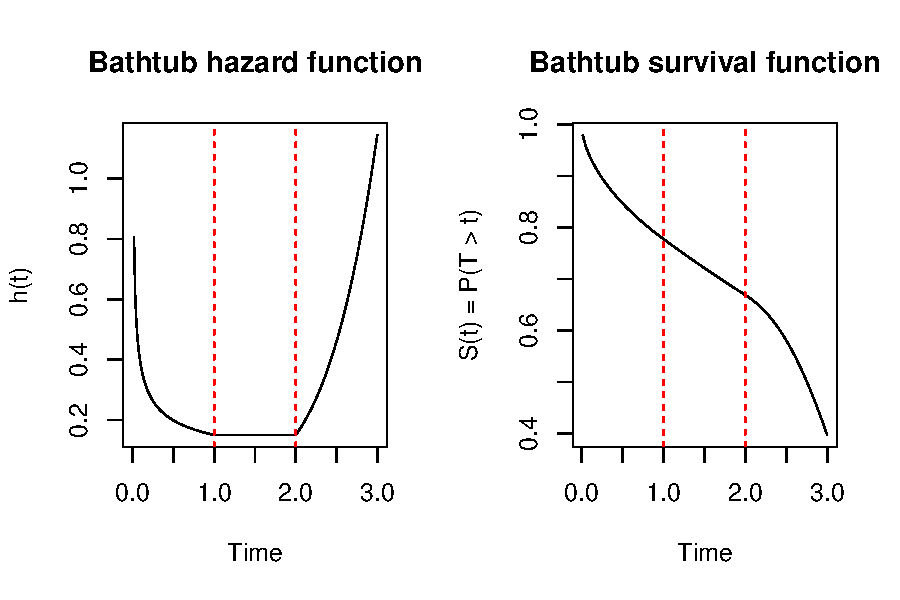
\includegraphics{fig-background/bathtub.pdf}
  \caption{An example of a bathtub hazard function (left) with the corresponding survival function (right). The dashed red lines indicate $t_1$ and $t_2$, the points in time when the nature of the hazard function changes. \label{Fig:bathtub}}
\end{figure}
Athena incorporates additional details into the hazard function. Performing maintenance tasks extends the expected life of a subassembly, whereas operator misuse decreases lifetimes, and the probability of operator misuse decreases with time, reflecting increased experience. A concept known as `virtual life' allows us to further manipulate $h(t)$. If we replace $t$ by $v(t)$, the virtual life, the hazard function, $h(v(t))$, can then reflect the state of the subassembly it models more accurately. We can think of $v(t)$ as the effective age of a component. Performing preventative maintenance should improve the lifespan of a component, thus it is effectively a `newer' component than prior to maintenance \citep{Finkelstein2007}. A driver of subassembly lifetime is the onset of ageing, that is, the start of phase (iii) of the hazard function.

In practice, the values of many model parameters in Athena are unknown, thus uncertainty distributions are to be elicited from experts and propagated through Athena to understand how input uncertainty induces uncertainty in key metrics.
A key model output is a time series which tracks the ``availability'' of a wind farm over time. Availability is a measure of reliability (performance) of offshore wind farms; the availability at time $t$ is the energy output of the wind farm as a proportion of the maximum possible energy output at time $t$. In \cref{Fig:availability-trajectories} we show a collection of $300$ availability trajectories, from a variant of Athena which is explained in \cref{Sec:athena-variant}. We see two modes in this particular collection. The main mode exhibits trajectories that never appear to drop below $0.8$. The lesser mode consists of trajectories which decrease shortly after the wind farm begins operation and do not start recovering until $2.5$ years of operational life has passed. After $3.5$ years, the trajectories all exhibit stable behaviour, apart from one trajectory which drops below $0.9$; this is due to a shortage of spare components.

Offshore wind farms have a mean availability of around $93\%$ for near shore turbines, but this is reduced for turbines further away from the coast since reaching the turbines for repair is much more difficult \citep{Carroll2016}. Availability is related to a wind farm's uptime and hence its profitability.
\begin{figure}[ht]
	\centering
	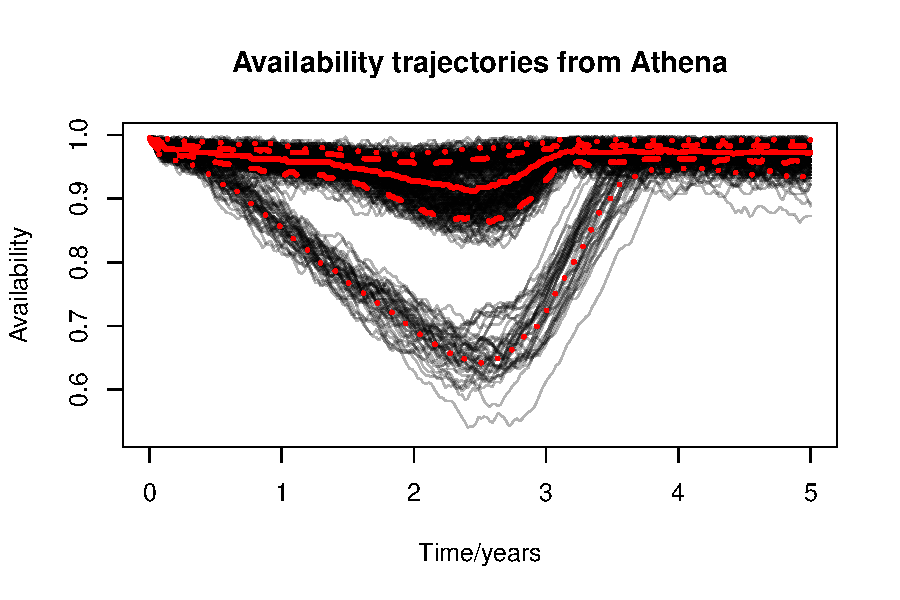
\includegraphics{fig-background/trajectories.pdf}
	\caption{A collection of $300$ typical availability trajectories (black lines) over the first $5$ years of a wind farm's operational life for a fixed set of parameter values. The solid red line represents the point-wise median trajectory, the dashed red lines represent $20^{th}$ and $80^{th}$  point-wise percentiles and the dotted red lines represent $5^{th}$ and $95^{th}$ point-wise percentiles.}
	\label{Fig:availability-trajectories}
\end{figure}
 In the first $5$ years of operation, \textit{excessive failure} is frequently observed. That is, the wind farm typically under-performs due to higher than expected numbers of component failures; tackling this issue is vital to the feasibility of offshore wind.

\subsection{A variant for spare components \label{Sec:athena-variant}}

The above description of the Athena simulator assumes that, when a subassembly suffers a failure that warrants replacement, rather than repair, that a replacement component is immediately available. In practice, this is an unrealistic assumption. Improving upon this assumption is necessary for our analysis in \cref{Ch:ds-for-ow}. A minor contribution of this thesis is some additional modelling within Athena to incorporate spare components and implementing this as simulator code.

A practical workaround to the problem of subassemblies being difficult to obtain, is to pre-order spare subassemblies and store them in a warehouse that is onshore, but close to the offshore wind farm. Within the Athena simulator, a subassembly can experience one of three types of failure. These are minor, moderate and severe failures. We have assumed that minor and moderate failures are of a nature such that they can be repaired with readily available tools or components. Severe failures are such that replacement of the subassembly is the only feasible option. We assume spare components are stored in a warehouse, which holds a fixed number of spare parts. At the start of the simulation, the user must choose how many of each spare part the warehouse can hold. These numbers are fixed for the entire simulation period. Denote the maximum number of spare subassemblies of type $i$ by $s_i$. Now let $s_i(t)$ be the number of spare parts we have available of type $i$ at time $t$. In essence, we have a finite number of spare parts readily available, which may be replenished at some future time.

Now suppose that a subassembly of type $i$ has suffered a serious failure. If there is a readily available spare part, then the part is shipped out to the turbine and it is repaired according to the processes within the `standard' version of the Athena simulator (so we still need the correct type of boat to be available, for example). If no spare part is available, because all the spares of type $i$ have been used, then the repair cannot take place until a new batch of spare parts arrives. This motivates a mechanism for ordering in more spare parts. We define a threshold, $s'_i$ such that, as soon as $s_i(t) < s'_i$, an operator within the wind farm places an order for more spare components. The $s'_i$ are specified at the start of the simulation and remain fixed for a given run of the simulator. The waiting time for the order is uncertain. If the order is placed at time $t$ then the order arrives at time $t + \Delta t$ where $\Delta t \sim Gamma(w_1, w_2)$, where $w_1$ and $w_2$ are uncertain parameters which could be elicited or specified by an expert.

There is also an extra mechanism regarding spare parts. It may be the case that the supplier cannot fulfil the order, or the order is only partially completed. We model the number of ordered spares that can actually be delivered, $s$, by a Binomial distribution; $s \sim Binomial(s_i - s_i(t), p)$. We would imagine that commonly, the order would be completely fulfilled. In such a case we can choose $p$ to be quite large, for example, $p = 0.99$. Whether an order can be fulfilled or not follows a Bernoulli distribution. We introduce a random variable $\omega \sim Bernoulli(p')$ where $p'$ is the probability that an order is fulfilled. $p'$ would typically take a large value, such as $0.99$. The total number of spares delivered from the order is then $s\omega$, and this is delivered at time $t + \Delta t$.

This concludes our introduction to the Athena simulator. We have introduced the necessary details for the applications later in this thesis, although more details can be found at \citet{Zit13, Zit16, Zit2021}.

\section{Elicitation of probability distributions \label{sec:prob}}

When quantities are unknown, and there is a lack of relevant data to estimate them, a feasible solution is to elicit them from an expert, or group of experts. Elicitation is the act of turning the knowledge or beliefs an expert has about unknown quantities into a joint probability distribution.

The elicitation of uncertain inputs, although useful when there is a lack of relevant data (or necessary if we wish to perform a Bayesian analysis utilising genuine prior beliefs), is a time consuming task which needs to be done carefully.

\subsection{The basics of elicitation}
In the elicitation process there are two roles. First we have the \textit{expert}. This is the individual whose knowledge or beliefs we aim to elicit and represent via a probability distribution. The term `expert' refers to their domain knowledge and expertise and has no reflection of their knowledge of statistics or probability. Commonly we will refer to multiple experts rather than singular; it is encouraged to combine the beliefs of multiple experts into a single distribution. The second role is the \textit{facilitator}; this a person who has good knowledge of probability and statistics, they guide the expert through the elicitation process and fit distributions to the elicited quantities.

Elicitation of a single uncertain quantity, $\theta$, is described as a four stage approach by \citet{Garthwaite05}.

The first stage is setting up the elicitation; this involves identifying an expert (or even a group of experts, as in \citet{Williams2021}), providing the experts with training and identifying precisely what $\theta$ is. By precisely, we mean that if $\theta$ is the rate at which the a gearbox, of brand X and model Y, would degrade at an offshore wind farm at location Z, then the experts should be told that $\theta$ is this value, rather than just ``the rate at which a gearbox degrades''.

The second task in the process is the `main' elicitation step: the expert states various summaries about $\theta$. Summaries are typically of the form $\p (a_i < \theta < b_i) = p_i$, $i = 1, 2, \ldots, n$. The facilitator can then fit a statistical model to the elicited $(a_i, b_i, p_i)$. In some cases we might be able to do this exactly and analytically. For example, if we elicit two quantities and assume $\theta \sim \mathcal{N}(\mu, \sigma^2)$, we can find $\mu$ and $\sigma$ via a pair of linear simultaneous equations in $\mu$ and $\sigma$. More generally, if there are more $p_i$ than parameters of the chosen distribution, or the form of the distribution does not lend itself to a tractable solution, then a numerical approach, \correction{such as minimising $T(\varphi) = \sum_i (p_i - \p (a_i < \theta < b_i \mid \bm{\varphi}))^2$ may be appropriate, where $\bm{\varphi}$ are the parameters of the distribution to be fitted.} This stage, and the previous stage, of fitting are somewhat interrelated; the form of the distribution the facilitator may wish to fit to the expert's beliefs may influence the questions asked. For example, when eliciting a distribution for a proportion, a Beta distribution, $\theta \sim Beta(\alpha, \beta)$, offers an appropriate model. Knowing that we will fit a Beta distribution to the elicited information means we would never ask the expert for $p_i$ such that $p_i = \p (5 < \theta < 50)$.

The `final' stage is then checking the adequacy of the fitted distribution. In this stage, the facilitator may show the expert what their elicited statements imply about $\theta$. If these statements are inconsistent with the expert's beliefs, we must go back and forth between the second, third and fourth stages until the expert and facilitator agree on a distribution, $\pi(\theta)$, which is an appropriate description of the expert's beliefs.

We have excluded the details about what kinds of questions a facilitator should ask the expert in order to obtain summaries of $\theta$. For guidance on the exact phrasing of questions, see \citet{Ohagan06}, in particular, Chapter $5$. Note that the types of questions to be asked are often related to the nature of the uncertain quantities, thus the general recipe for elicitation is necessarily vague. Some further practical guidance is given in \citet{Kadane1998}, who advocate for eliciting \textit{observable} quantities rather than the parameters of any statistical model. An observable quantity is, as its name suggests, a quantity that can be observed by the expert. This means we should ask experts about the quantities exhibited by a physical system (for example, a time to failure of a component in the wind farm), rather than parameters of a statistical model (for example, the parameters of a Weibull distribution).

\subsection{The Sheffield Elicitation Framework}
A popular elicitation procedure, the Sheffield Elicitation Framework (SHELF), provides a thoughtful routine for eliciting an unknown quantity from one or more experts. The procedure can be applied to a single expert, but we adopt the convention of multiple experts. SHELF is also used for multiple uncertain quantities, which we describe later.

SHELF consists of a collection of documents, which includes forms and presentation slides \citep{SHELF4}, this is accompanied by software to fit distributions to elicited beliefs, as well as validate them \citep{SHELFpkg}. Both the software and documents are designed to help the facilitator and the experts elicit an uncertain quantity of interest. SHELF covers all aspects of the elicitation process, from the recruitment of experts, to the `main' elicitation step, as well as checking the adequacy of $\pi(\theta)$ as a representation of the expert's knowledge of $\theta$. An important concept in SHELF is RIO: the rational impartial observer. RIO is a hypothetical fly on the wall who, if they had no strong beliefs about $\theta$ prior to observing the discussion amongst experts, would hold beliefs characterised by $\pi(\theta)$ after observing their discussion. The experts are instructed to formulate a distribution, $\pi(\theta)$, which summarises the knowledge of all the experts. This combined judgement does not have to be an equal weighting of each individual's beliefs; the experts are free to give more consideration to more knowledgeable experts as they see fit.
The core elicitation step is broken into two main parts; individual elicitation and a group elicitation as follows:\footnote{We have condensed the steps considerably. We aim to communicate the core steps in SHELF rather than replicate the documentation.}
\begin{itemize}
\item[1.] {Conduct an individual elicitation for each expert as follows:}
  \begin{itemize}
    \item[(i)] Specify a lower value, $L$, such that the event $\theta < L$ is `extremely unlikely'. By `extremely unlikely', it is meant that if you were to learn that $\theta < L$, your initial reaction would be that the statement $\theta < L$ is false. Repeat the process for an upper limit, $U$, where the event $U>\theta$ is extremely unlikely.
    \item[(ii)] Elicit the median, $m$ such that $p(\theta < m) = 0.5$. $m$ is the value that placing a bet on $\theta < m$ has an equally desirable outcome to placing a bet on $\theta \geq m$.
    \item[(iii)] Elicit a lower quartile, $Q_1$ such that $\p(L \leq \theta < Q_1) = \p(Q_1 \leq \theta < m) = 0.25$. As above, placing a bet on the event $L \leq \theta < Q_1$ should be equally desirable to placing a bet on the event $Q_1 \leq \theta < m$.
    \item[(iv)] Elicit an upper quartile, $Q_3$ such that $\p(m \leq \theta < Q_3) = \p(Q_3 \leq \theta < U) = 0.25$. This step is similar (iii).
    \item[(v)] The facilitator now fits a distribution to the elicited knowledge, treating the limits, quartiles and median as data.
  \end{itemize}
\item[2.] {Conduct a group elicitation as follows:}
  \begin{itemize}
    \item[(i)] As a group, perform all the steps in part 1.
    \item[(ii)] Verification: is the fitted distribution what a RIO would conclude as appropriate?
  \end{itemize}
\end{itemize}
This process is what we will describe as a `full SHELF' elicitation. Step $1. (v)$ can be performed in a semi-automatic way via the \texttt{SHELF::elicit()} function, which opens a Shiny app. The facilitator fills out boxes within the app corresponding to elicited information. The app can either fit a single chosen parametric form, or try many parametric forms and return the form which offers the closest fit to the elicited beliefs. A screenshot of the app is given  in \cref{Fig:shelf-app}. In the example, the elicited information leads to $\log \theta \sim t_{10}(6.02, 0.5)$, where $\theta$ is the number of coffees consumed in the production of this thesis and $t_\nu (\mu, \lambda^2) = \mu + \lambda t_\nu$ is a location-scale variant of the $t$ distribution.
\begin{figure}
  \centering
  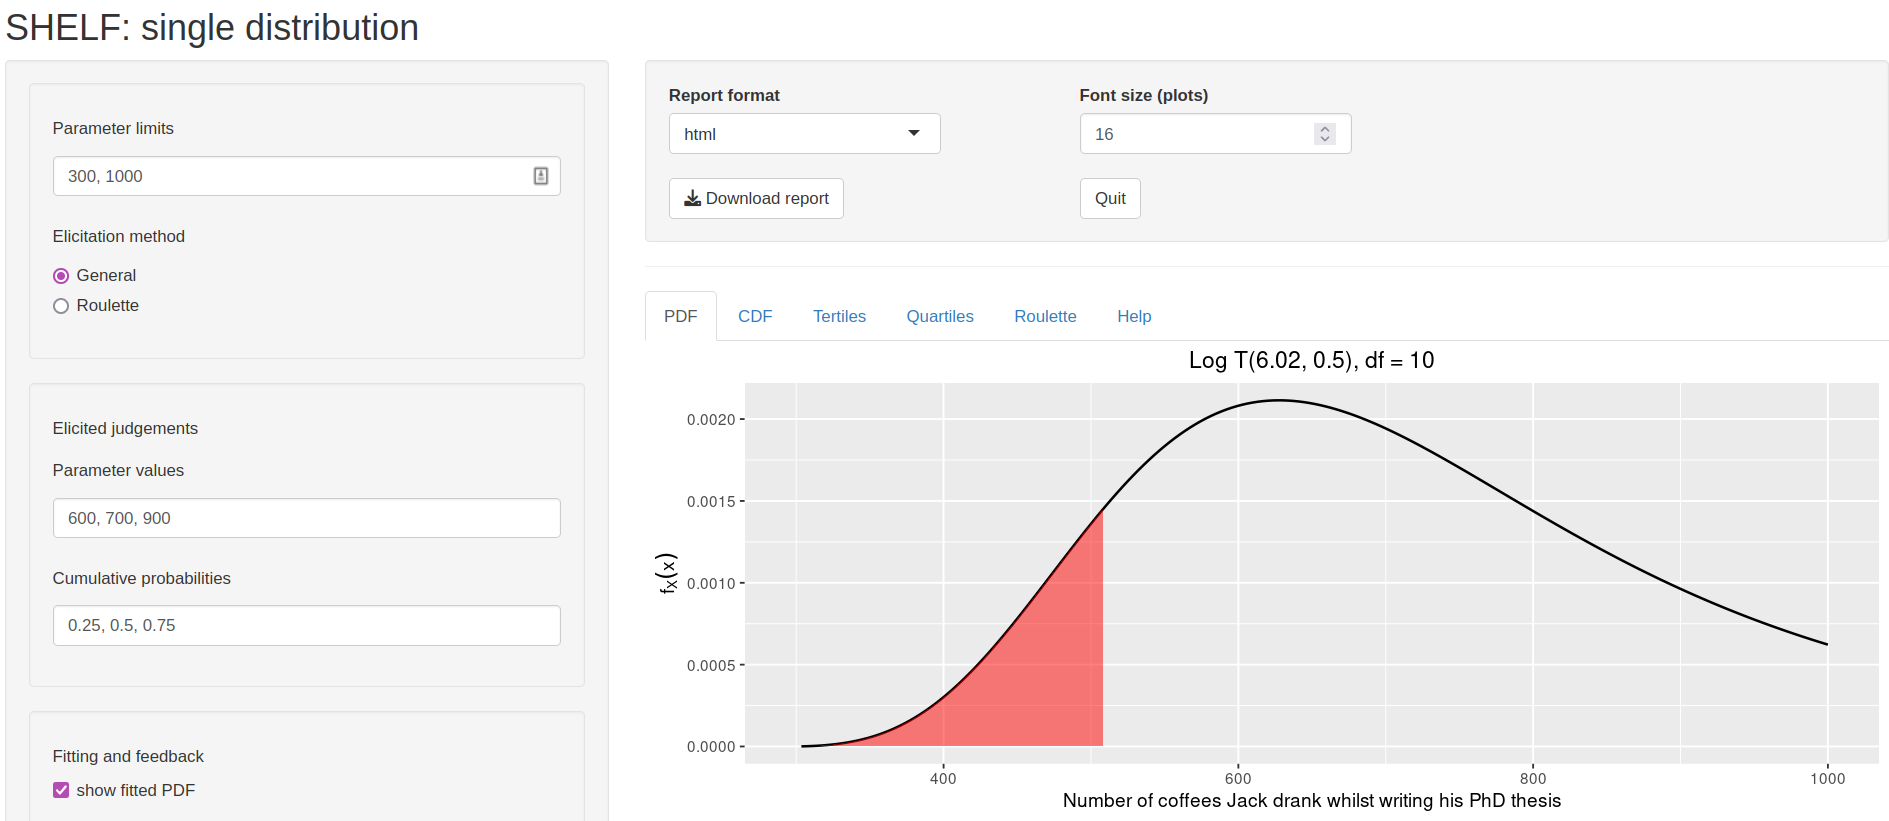
\includegraphics[width=\textwidth]{fig-background/shiny.png}
  \caption{Screenshot of distribution fitting functionality provided by the \texttt{SHELF} package \citep{SHELFpkg}. In this particular example, we have elicited the number of cups of coffee the author of this thesis believes he has drunk in order to complete this thesis. The red shaded area represents a feedback question.\label{Fig:shelf-app}}
\end{figure}
\subsection{Elicitation of many uncertain quantities}

Suppose we have $k>1$ uncertain quantities, $\btheta = (\theta_1, \theta_2, \ldots, \theta_k)^T$. We wish to characterise uncertainty about $\btheta$ via $\pi(\btheta)$, a joint density. If the expert is willing to assert that $\theta_i \indep \theta_j \,\forall\, i \neq j$, then we may write $\pi(\btheta) = \prod_{i=1}^k \pi_i (\theta_i)$. In this case, all we need to do is elicit $\pi_i(\theta_i)$ using the univariate method outlined above.

If the components of $\btheta$ cannot be assumed to be independent there are two approaches within SHELF. The first is to rephrase the problem in terms of new unknowns, $\btheta'$, such that $\theta'_i \indep \theta'_j \,\forall\, i \neq j$. For example, suppose we are planning the programme for a statistics conference, we may want to elicit
\begin{itemize}
  \item[(i)] $\theta_1 = \text{the number of delegates at a particular statistics conference}$
  \item[(ii)] $\theta_2 = \text{the number of delegates at the conference who are Bayesian}$.
\end{itemize}
Clearly, $\theta_1 \geq \theta_2$, thus a dependence is present. Now let $\theta'_1 = \theta_1$ and $\theta'_2 = \theta_2/\theta_1$, that is, the proportion who are Bayesian. The statement $\theta_1' \indep \theta_2'$ seems more plausible than $\theta_1 \indep \theta_2$. We recover $\btheta$ via $(\theta_1, \theta_2)  = (\theta'_1, \theta'_1 \theta'_2)$.

The second approach is to try to elicit the dependence between elements of $\btheta$. This is a much more challenging task than assuming independence, thus should only be done when necessary. Within SHELF, dependence may be elicited via assuming an appropriate distributional family that lends itself well to dependence (for example, multivariate Normal or Dirichlet). The second option is to incorporate dependence via a copula. A copula is a useful device for constructing a dependence structure between two random variables with known marginal distributions \citep{Bedford2014, Elfadaly2017}. In either case, we must elicit marginal distributions and the dependence structure.

Eliciting even the marginal distributions can take a long time. The European Food Safety Authority (EFSA) state that elicitation of a single unknown takes about a day \citep{EFSA2014}. EFSA believe that elicitation of $4$--$6$ parameters takes about $2$ days. The experts are able to perform elicitation more quickly because they become accustomed to the process. Elicitation workshops are time limited for practical reasons. The first is that experts will become fatigued, thus after several days their judgements degrade in quality. The second is that experts will only be available for a limited amount of time; they will have other commitments. We may only have access to the experts for a day or so. For this reason, we must think carefully about which parameters deserve a full SHELF treatment and which parameters require less thought. This amounts to different types of elicitation. The most rigorous is the full SHELF treatment, reserved for the most important parameters.

An approach that is less involved than SHELF, but retains many of its features is probabalistic Delphi \citep{Rowe1999}, which can take place remotely (for example, via email).  A questionnaire about unknowns, with questions similar to that found in a full SHELF workshop, is sent to experts, which they return to the facilitator. The questionnaire responses are then circulated anonymously amongst all experts so they can review the other opinions about $\btheta$ and revise their own beliefs as appropriate. The revised beliefs are sent to the facilitator who then uses a mathematical aggregation rule --- such as a linear combination of each expert's $\pi(\btheta)$ --- to combine each expert opinion into a single distribution.

A less sophisticated, but much less time consuming, approach would be to employ a `minimal assessment'. Minimal assessment may proceed by eliciting $L$ and $U$ from each expert, then for the facilitator to assume a very simple form for $\pi_i(\theta_i)$. For example, we might take $\theta_i \sim \mathcal{U}(L, U)$. Another simple form would be $\theta_i \sim \mathcal{N}(\mu, \sigma^2)$  with $\mu = \frac{1}{2}(L+U)$ and $\sigma = \frac{1}{2}(U-\mu)$ (remembering that $95\%$ of a Normal distribution's mass lies within $\pm 2 \sigma$  of  $\mu$). Each expert's $L$ and $U$ could be revised via a Delphi-like approach, or the facilitator could take $L^{*} = \min{L}$, $U^{*} = \max{U}$ and fit a distribution based on $U^{*}$ and $L^{*}$. A minimal assessment is often employed when we want to use expert judgement for a prior in a Bayesian analysis, but we know that a reasonably large sample of data is available. The sample will be sufficiently large to dominate any prior specification, thus we choose not to worry about precise details of $\pi(\btheta)$.

How we choose which parameters warrant a full SHELF treatment and which parameters require a less formal treatment can be dealt with via a sensitivity analysis. In almost all cases, the distribution $\pi(\btheta)$ is not of direct interest. We are usually interested in the distribution $\pi(\btheta)$ induces on $f(\btheta)$, a function of the uncertain parameters. Concretely, we may want to propagate uncertainty about model parameters, $\btheta$ through a complex model (such as the Athena simulator) to make predictions about quantities relevant to decision making, such as the availability time series,  or summaries of it. The SHELF documentation suggests that a one-way sensitivity analysis may be appropriate. In this case we study how much $f(\btheta)$ changes when $\theta_i$ is perturbed to $\theta_i \pm \Delta \theta_i$. How much $f(\btheta)$ changes when only $\theta_i$ changes is a simple, but limited, way to investigate the relative importance of each $\theta_i$. In \cref{Ch:sensitivity} we give an in-depth discussion of sensitivity analysis, the relative importance of parameters, and best practices for sensitivity analysis with a view towards eliciting uncertain parameters of a model.

\section{Decision analysis \label{sec:decision}}

Unless explicitly stated otherwise, this section is based upon \citet{Keeney1976}, \citet{Smith2010} and chapters of \citet{ElicitationBook}; in particular \citet{Gonzalez2018}.

In many of the decision making situations we encounter in our lives, our idea of the `best' decision may differ to another person's idea about what is the `best' decision. Consider the problem of preparing a scone to be eaten. One individual may claim that putting jam on a scone \textit{before} the cream is objectively the best method to prepare it. Many other people would express dogmatically that the cream \textit{must} be first. Others would argue that the best way is not defined by the ordering of cream or jam, but much rather, the quantity of cream and jam.

These differences are present because every decision maker (DM) has their own preferences. Much like how we all have different prior beliefs for an unknown quantity, we also have different preferences for outcomes and thus different optimal decisions. A DM's preferences are expressed via a utility function which can be elicited from the DM. This function can have different shapes for different DMs. In fact, different DMs may have utility functions which have different inputs. We will now formalise the notion of a utility function.

Let $\calX$ represent the set of all possible decisions the DM could make, and let $\bx \in \calX$ be a single decision. Further suppose that any relevant unknown quantities, $\btheta$, within the decision problem have been assigned a probability distribution $\btheta \sim \pi (\btheta)$. In this thesis $\pi(\btheta)$ will usually be an elicited prior distribution, but it should be replaced by the posterior distribution $\pi(\btheta \mid \by)$ when relevant data $\by$ are available. Finally, we need a function $u(c(\bx, \bphi))$ which is a mathematical representation of the DM's beliefs for how desirable the consequence $c(\cdot, \cdot)$ is when decision $\bx$ has been made and when $\btheta$ takes the value $\bphi$. The function $c(\cdot, \cdot)$ may be deterministic when it is clear how decisions impact future events, or it can be a stochastic function when future events are uncertain.

The optimal decision is given by
\begin{equation}
  \bx^{*} = \argmax_{\bx \in \calX} U(\bx). \label{Eq:opt-dec}
\end{equation}
where
\begin{equation}
U(\bx) = \E_{\btheta} \{ u(c(\bx, \btheta)) \} \label{Eq:exp-util}
\end{equation}
is the expected utility of the decision $\bx$. The expectation in \cref{Eq:exp-util} depends on several things:
\begin{itemize}
  \item[(i)] $\pi(\btheta)$, the probability distribution over all relevant unknown quantities
  \item[(ii)] $c(\bx, \btheta)$, the \textit{consequence} of decision $\bx$ when the unknown quantities take the value $\btheta$.
  \item[(ii)] $u(c(\cdot, \cdot))$, the utility function describing how preferable a consequence is. Larger values of $u(c(\cdot, \cdot))$ indicate more preferable consequences.
\end{itemize}

For many problems, an `off the shelf' utility function may adequately describe our preferences. For example, in Bayesian design of experiments, the goal is often to choose a design $\bx \in \calX$ which allows us to learn the most about some unknown quantities. One appropriate, default utility function is the Kullback-Leibler divergence between the prior and posterior distributions for the unknowns. A review of appropriate utility functions for Bayesian design of experiments is given in \citet{Ryan2016}.

For many practical problems, there are many competing objectives which may not be well defined. For example, we would typically want to maximise energy output of the wind farm, and simultaneously minimise operation and maintenance costs. These objectives compete with each other. Increasing maintenance costs may increase energy generation, for example. A less well defined objective is keeping local residents happy with the development of the offshore wind farm, in such a case we must come up with a \textit{proxy} for resident discontent which we can observe. The DM may wish to re-phrase resident discontent as the number of local residents who sign a petition against the development of an offshore wind farm, for example.

Since the development of an offshore wind farm is a highly specialised problem, it is unlikely that an off the shelf utility function will describe the objectives we wish to achieve. Further, different decision makers may have different preferences. For example, the CEO of an energy company may be mainly motivated by profits, whereas, a systems safety engineer's first priority is the safety of those maintaining the wind farm. Therefore, once a DM has been chosen, we need to encode their unique preferences into a utility function. This is done by \textit{eliciting} the utility function, $u(\cdot)$ from the DM. We must also elicit $\pi(\btheta)$. We do this via the methods given in \cref{sec:prob}.

We now provide an overview of some utility elicitation techniques. This allows us to turn an ill-defined decision problem into the well-posed questions of mathematical optimisation.

\subsection{Fundamental notions of utility}

There are three axioms of utility theory under risk, where a preference relation $\preceq$ is assumed on a probability space $\mathcal{P}$. To discuss the fundamental notions of utility we need to define a \textit{lottery}. A lottery, $p = [x, y; r]$ is an uncertain event where $p = x$ with probability $r$ and $p = y$ with probability $1-r$. For lotteries $p$ and $q$ the statement $p \preceq q$ means that $q$ is \textit{at least} as desirable as $p$. \correction{The statement $p \prec q$ means that $q$ is more desirable than $p$.}

The three axioms are as follows:
\begin{enumerate}
\item \textbf{Weak order:} $\preceq$ on $\mathcal{P}$ is complete; $\forall$ $p, q \in \mathcal{P}$ either $p \preceq q$ or $q \preceq p$ and is transitive; $\forall p, q, r \in \mathcal{P}$  $p \preceq q$ together with $q \preceq r$ $\implies$ $p \preceq r$.

\item \textbf{Archimedian:} $\forall p, q, r \in \mathcal{P}$ if $p \prec q \prec r$ then $\exists \alpha, \beta \in (0, 1) $ such that $\alpha p + (1-\alpha)r \prec q \prec \beta p + (1-\beta) r$.

\item \textbf{Independence:} $\forall p, q, r \in \mathcal{P}$ and $\alpha \in (0, 1]$, $\alpha p + (1-\alpha)r \preceq \alpha q + (1-\alpha) r \iff p \preceq q$.
\end{enumerate}
Under these conditions there is a \textit{utility function}, $u$, satisfying $\forall p, q \in \mathcal{P}$
\begin{enumerate}
\item[(i)] $p \preceq q \iff u(p) \leq u(q)$
\item[(ii)] $u(\alpha p + (1-\alpha) q) = \alpha u(p) + (1- \alpha)u(q)$.
\end{enumerate}
From this, we can deduce $p \preceq q \iff \E_p(u) \leq \E_q(u)$, where $\E_p(u)$ is the expected utility of a lottery $p$.

Note that a utility function is only unique up to a positive affine transformation; $au(\cdot) + b$, for any $a >0$ and $b \in \mathbb{R}$, represents the same set of preferences as $u(\cdot)$.

\section{A basic single attribute utility elicitation}

One of the first steps in a decision analysis is to decide what we measure to decide how good a decision is. The attribute is the quantity that we measure to describe how preferable a decision is. Common attributes would be financial gain in a business setting or whether an individual recovers from surgery in a medical setting. The consequence is the realised value of an attribute after making a decision.

When eliciting a utility function for an uncertain consequence, $c(\cdot, \cdot)$, it is much easier to consider trade-offs under certainty. We therefore elicit the utility function as a function of consequences $c$ rather than decisions $\bx$ and unknown states $\btheta$. When finding the optimal decision, we revert to consequences being uncertain; that is, replace $c$ by $c(\bx, \btheta)$. We then calculate $\bx^{*}$ by optimising $U(\bx)$ (\cref{Eq:exp-util}) with respect to the decision, $\bx$.

A basic elicitation procedure is as follows. We assume that $u(c)$ is monotonically increasing in $c$.

\begin{enumerate}
	\item Determine $[c^0, c^*]$; the range for the attribute of interest. Assume $c^{0} \prec c^{*}$.
	\item Set $u(c^*) = 1 - u(c^0) = 1$.
	\item Elicit utilities $\{u_1, \ldots, u_n\}$ for a set of intermediate consequences $\{c_1, \ldots, c_n \}$.
	\item Fit a utility function to the quantities $\{(c^0, 0), (c_1, u_1), \ldots, (c_n, u_n), (c^*, 1) \}$. This can be done via a least squares procedure.
	\item Check for consistency; ask  the DM a few verification questions.
\end{enumerate}
The above recipe assumes a given functional form for $u(\cdot)$; choosing this functional form can be tricky. Further, assigning utility values to intermediate values is not trivial. It is also important to be aware of, and counter, the DM's inaccuracies and biases. If $u(c)$ is not monotonically increasing in $c$, the problem can frequently be rephrased so that $u(c)$ is monotonically increasing in $c$. For example, replacing $c$ by $-c$ when $u(c)$ is monotonically decreasing, or replacing $c$ by $(c - c')^2$ if $u(c)$ is increasing on $[c^{0}, c']$ then decreasing on $(c', c^{*} ]$.

The main step in the above procedure is step $3$: eliciting utilities for intermediate consequences. The number $n$ of utilities to be elicited will be a trade off between the accuracy of the resulting utility function and the time available.

There are two main ways to elicit $u_i$ in step $3$. The first is \textit{probability equivalence}. Here the DM must specify the probability $p$ where $[c^{*}, c^{0}; p] \sim c$ for a pre-determined consequence $c$. The notation $[c', c''; p] \sim c$ describes a lottery where $c'$ occurs with probability $p$, $c''$ occurs with probability $1-p$, and the uncertain result of this lottery is as desirable as the certain consequence $c$; that is $U([c', c''; p]) = U(c)$. The other way is to specify one of $\{ c, c', c''\}$ when $p$ and the other two elements of $\{c, c', c'' \}$ are determined. This is a \textit{certainty equivalence}.

Within each of the two main elicitation approaches, there are choices about how to specify probabilities and consequences. This concerns the choices of the multiple $c_i$ in the $(c_i, u_i)$ pair, or choosing related values of $p$ when constructing many certainty equivalences. Each of these has limitations, which are typically forms of biases, as well as advantages; see Section $10.2.2$ and Section $10.2.4$ of \citet{Gonzalez2018}, as well as references within for a discussion of the various biases that can occur when eliciting utilities and how to counteract them.
\subsection{Multi-attribute utility elicitation}
When eliciting a multi-attribute utility function (where the consequence space has $2$ or more dimensions), it is cognitively complex for the decision maker to simultaneously weigh up the relative merits of many consequences. For this reason, much like probability elicitation, the problem can be greatly simplified when certain notions of independence are assumed. The notion of independence we need is known as \textit{preferential independence}. Two (collections of) attributes $\mathcal{C}_i$ and $\mathcal{C}_j$, with $\mathcal{C}_i \cap \mathcal{C}_j =\emptyset$ are said to possess preferential independence if
\begin{equation*}
  (c_i, c_j) \succeq (c_i', c_j) \implies (c_i, c'_j) \succeq (c_i', c_j')
\end{equation*}
for some $c_j$ and all $c_j'$. \correction{We have introduced the symbol $\succeq$ which is similar to $\preceq$: $p \succeq q \iff q \preceq p$.} This type of independence allows the DM to specify judgements of the form \textit{``provided everything else is constant, I prefer X to Y''}. This allows us to elicit individual utility functions for each attribute $\mathcal{C}_i$ and then combine them to provide an `overall' utility function for all $m$ consequences, $\mathcal{C} = \mathcal{C}_1 \times \mathcal{C}_2 \times \ldots \times \mathcal{C}_m$. If preferential independence holds for all possible sets $i$ and $j$ then the DM views the consequences as \textit{mutually preferentially independent}. This is sometimes referred to as having \textit{mutually utility independent} consequences.
Now, assuming that consequences are mutually utility independent, there are two main ways to proceed. The first is to elicit a utility function which is a weighted sum of the marginal utility functions:
\begin{equation}
  u(c) = \sum_{i=1}^m w_i u_i(c_i). \label{Eq:add-util}
\end{equation}
This is appropriate when the DM's preferences between lotteries depends only on the marginal distributions over the $\mathcal{C}_i$ and not their joint distribution. If preferences depend on the joint distribution, then we should use a multiplicative form:
\begin{align}
  u(c) &= \sum_{i=1}^m w_i u_i(c_i)\label{Eq:mult-util}\\
        &+ k\sum_{i=1, j>i}^m w_iw_j u_i(c_i) u_j(c_j) \nonumber\\
        &+ \ldots  \nonumber\\
        &+ k^{m-1}w_1 w_2 \ldots w_m u_1(c_1) u_2(c_2)\ldots  u_m(c_m) \nonumber
\end{align}
where $w_i$ are weights to be elicited and $1 + k = \prod (1 + k w_i)$. The case $k = 0$ corresponds to the additive utility function in \cref{Eq:add-util}.

In the case of \cref{Eq:add-util} we can elicit the weights, $w_i$, by considering the consequence $c_{(i)}^0 = (c_1^0, c_2^0, \ldots, c_{i-1}^0, c_i^{*}, c_{i+1}^0, \ldots, c_m^0)$. $c_{(i)}^0$ is the consequence where all attributes are at their worst value, apart from the $i$th attribute which is at its best value. It is simple to verify that $u(c_{(i)}^0) = w_i$. This gives rise to an elicitation protocol where we cycle over the $c_{(i)}^0$ to obtain each $w_i$. Note that $\sum_{i=1}^m w_i = 1$ since the best consequence, $c^{*}$, satisfies $u(c^{*})=1$, and the worst consequence, $c^0$, satisfies $u(c^0) = 0$. This means only $m-1$ statements are required to elicit the $w_i$; additional statements can be used for verification. If the multiplicative form is used, one extra question needs to be asked. For example, we could invert one of the $c_{(i)}^0$ and have all but the $i$th consequence at its best value, and have the $i$th consequence at its worst value.

\subsection{Choosing functional forms for the $u_i$}

One of the most important issues is choosing the \textit{functional form} of the utility function. Two important features are: monotonicity (more profit is almost always preferred) and concavity (an assumption about the attitude to risk of the DM).

Suppose $C \in \mathbb{R}$ is a monetary consequence. For a lottery $p$ there are two expectations to consider. The \textit{expected utility} $\E_p[u(c)]$ and the expected (monetary) value $\E_{p} (c)$. The certainty equivalent, $c_p$ is the amount of money the DM would place on a single play of the lottery; $u(c_p) = \E_p(u(c))$. Equivalently, $c_p = u^{-1} \left\{ \E_{p} (u(c)) \right\}$.

The risk premium is defined to be the difference between the expected value of the lottery, and its certainty equivalent. We can interpret this as the difference in the value of infinite plays of the lottery versus a single play:

\begin{equation}
	\pi_p = \E_p (c) - c_p.
\end{equation}

The sign of $\pi_p$ is a result of the shape of $u$. $u$ is concave $\iff$ $\pi_p > 0$;  in such a scenario the DM is described as `risk averse'. An alternative phrasing of a risk averse attitude is preferring the average result from many plays of the lottery, to a single play of the lottery. A risk averse DM prefers a small deterministic payoff to a random payoff with larger expected value, but some chance of a very small payoff. This is common in financial situations. A risk prone DM ($\pi_p < 0$) will prefer the lottery to its expected consequence; a desperate individual may wish to spend their last $\pounds 1$ on a scratch card, since the prospect of winning thousands is much more appealing than the fact that they will probably lose their stake.

Of course, a decision maker does not have to be strictly risk prone or strictly risk averse. They could be risk neutral (in this case $u(x) = ax + b$ and $\pi_p  = 0$) or they could have a varying attitude towards risk. For instance, suppose the DM is a student who is planning their revision strategy for a pass/fail exam. Suppose the pass mark is $60\%$. When considering their revision strategy, the DM is willing to do almost anything that will get them above the pass mark. However, the DM is not desperate to achieve very high marks (although a very high mark would bring an increased level of personal achievement, which does increase the DM's utility of such events). For events below the pass mark, the DM will be risk prone, for events above the pass mark the DM will be risk averse; this leads to a sigmoidal shape. This is an example of the \textit{local} risk behaviour changing.

Choosing the best functional form from many candidate functional forms can be achieved by considering, for example, the sum of squares in the least-squares procedure used to find the parameters for any given functional form. Verification questions can also be used to see which functional forms are, or are not, consistent with the preferences of the DM. For example, we could ask the DM  for $c'$  such that $u(c')  = u'$, where  $u'$ is not close to any of the previously elicited $u_i$. If $u'$ is close to the fitted $u(c')$ then we would be comfortable with the fitted $u(c)$. If it is too far away, we should consider alternative functional forms, or even re-elicit the $(c_i, u_i)$ pairs. We should also verify with the DM, once we have constructed and optimised $U(\bx)$, that $\bx^{*}$ is a decision they would be willing to take. If $\bx^{*}$ is not a decision that the DM is willing to take, this suggests that somewhere in the process there has been an error, or the DM has changed their preferences. In such cases, we must go back to the start and re-elicit all attributes and functional forms.

\section{Discussion}

We have outlined some relevant background material to set the scene for the rest of this thesis.

We have introduced the Athena simulator, a stochastic point-process model used to make statements about the reliability of an offshore wind farm, with a view towards making decisions about the operations and maintenance of the wind farm. The Athena simulator is typical of many simulators within the wider area of reliability analysis as it is stochastic, expensive and relies on many uncertain parameters. This makes the Athena simulator a suitable example for extensive case studies within later chapters.

We then discussed one approach that a subjective Bayesian may use to elicit a (joint) probability distribution. This approach is known as SHELF. We discussed that elicitation is useful when there is a lack of relevant data, although it is not a trivial procedure. We must take great care to elicit an honest and faithful representation of the beliefs experts possess. SHELF promotes the use of sensitivity analysis to gauge the relative importance of each element of $\btheta$, in order to obtain the most useful belief specification about $\btheta$ in the time available.

Finally, we introduced some basic concepts of decision making, such as utility, as well as motivating subjective utility functions as ways to capture the preferences of a DM and the trade-offs that they must make in complex problems. We discussed some approaches to eliciting multi-attribute utility functions by comparing a given lottery to certain consequences. We discussed ways to combine given marginal utility functions into a multi-attribute utility function. We also discussed aspects of choosing the functional form of the marginal utility functions.
\end{chapter}
